%!TEX root = ../Thesis.tex


\section{Test}

\subsection{Testklassen \textcolor{blue}{[Jonathan Brockhausen]}}

Als Testframework haben wir JUnit verwendet. Wir haben dedizierte Testklassen, in denen wir die relevantesten Teile der geschriebenen Programmlogik mit Tests abdecken können. Wie in \cref{Arbeitskonzept} bereits geschrieben wurde, können wir durch die Einbindung der GitHub CI eine Sicherstellung der Funktionalität erreichen.
Im Folgenden werden die konkreten Testklassen und die Abdeckung erläutert. Die Testabdeckung der Kern-Anwendung ist in \cref{fig:coverage} dargestellt.

\begin{figure}[h!!]
    \centering
    \begin{minipage}[t]{1\textwidth}
        \caption{Testanwendung der Kern-Anwendung}
        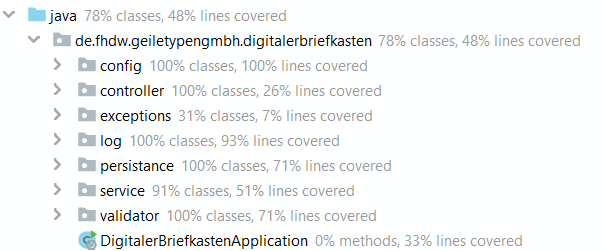
\includegraphics[width=1\textwidth]{img/coverage.png}\\
        \source{Eigene Darstellung}
        \label{fig:coverage}
    \end{minipage}
\end{figure}

Insgesamt erreichen wir eine Testabdeckung von 78\%. Von den Tests wird nahezu die gesamte Funktionalität des Programms abgedeckt. Elemente, die nicht getestet werden, sind im wesentlichen die Exceptions und Teile der Controller, in denen beispielsweise das funktionell identische Anlegen von Produktsparten, Zielgruppen, Vertriebskanälen und Handlungsfeldern nur einmal stellvertretend getestet wird.

Die Tests sind auf zwei Klassen aufgeteilt, \texttt{IdeaControllerIntegTest} und \texttt{UserControllerIntegTest}. Wir trennen damit die Integrationstests von Ideen- und Benutzerfunktionalität voneinander. In beiden Testklassen wird zunächst mit Helfermethoden die Testumgebung vorbereitet indem Objekte und Klassen geschaffen werden, die von den Tests genutzt werden.
Die tatsächlichen Testmethoden sind jeweils sprechend benannt und benutzen größtenteils die vom Spring-Framework bereitgestellten MockMvc-Funktionalitäten um gemockte Anfragen zu senden und die Antworten auszuwerten. Die einzelnen Tests testen jeweils eine vollständige Funktionalität des Programms. Es kann mehrere Tests geben, die eine Funktionalität mit deren Abwandlungen testen.
Aufgrund des logisch zusammenhängenden Aufbaus der Testklassen und -Methoden wird auf eine detaillierte Erläuterung verzichtet.

\subsection{manuelle-\enquote{Klicktests} \textcolor{blue}{[Julius Figge]}}

Zur Überprüfung der GUI sollen manuelle Klicktests durchgeführt werden.
Diese sollen dokumentiert werden um Fehler möglichst gezielt beheben zu können.\\

\subsubsection*{Zu notierende Informationen}
Für die Auswertung relevant sind zum einen die Programmrevision (Git Commit Hash, Datum) sowie der verwendete Branch. Darüber hinaus ist das genutzte Betriebssystem sowie der genutzte Browser (inklusive Build zu notieren).
Bei Darstellungsfehlern ist es sinnvoll, zudem Screenshots zu hinterlegen sowie die Bildschirmauflösung zu notieren.
Diese Informationen sammeln wir gezielt sehr detailliert, um Fehler besser eingrenzen zu können.

\subsubsection*{Testvorbereitung}
\begin{enumerate}
    \item Zum Testen wird der neueste Stand des Master-Branches verwendet.
    \item Hierzu ist zunächst die Datenbank zu löschen und mit Hilfe der in \enquote{HelperScriptsNoTests}        vorhandenen Tests zu füllen.
    \item Der Code soll kompiliert werden und die entstandene \enquote{Jar}-Datei ausgeführt werden.
    \item Nach Möglichkeit soll der Test auf mehreren Browsern ausgeführt werden. Hierbei ist zu beachten, dass alle Addons zu deaktivieren sind, um eventuelle Komplikationen auszuschließen.
    \item Die Entwicklerkonsole ist zu öffnen um hier enstehende Fehler und Warnungen mit in die Testergebnisse aufzunehmen.
    \item Nachdem diese Voraussetzung geschaffen ist, sind die Tests durchzuführen und die obigen Informationen zu notieren.
\end{enumerate}

Zur Testdurchführung ist die Tabelle im Anhang \ref{fig:testdurchf} auf S.\pageref{fig:testdurchf} zu verwenden.

